% https://ask.latexstudio.net/ask/question/17406.html
\documentclass[margin=1.5cm]{standalone}
\usepackage{tikz}
\usepackage{amsmath}
\usetikzlibrary{positioning,calc,intersections}
\begin{document}
    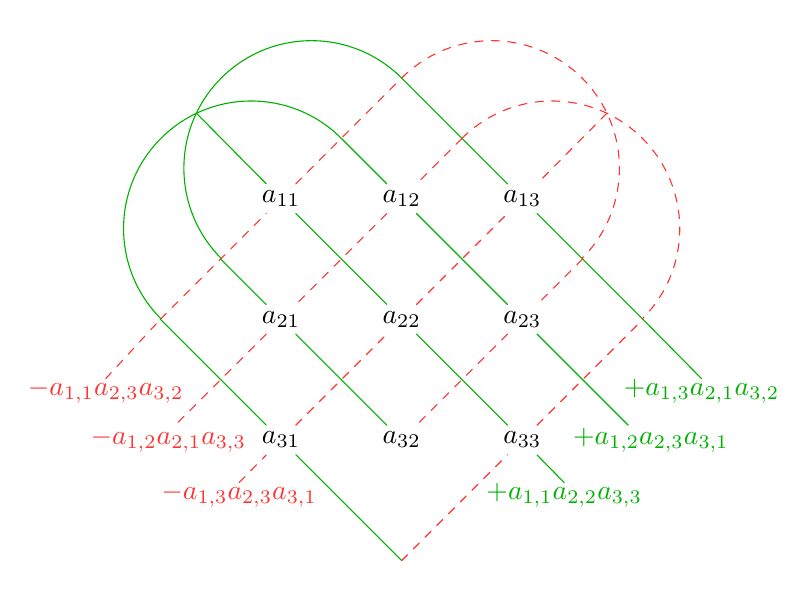
\begin{tikzpicture}[
        every node/.style = {circle,outer sep=0pt,inner sep=.1pt},
        lineleft/.style = {color = red!80,dashed,line cap=round},
        lineright/.style = {color = green!70!black,line cap=round},
        ]
        \node (node-22) {$a_{22}$};
        \node (node-21) [left = of node-22] {$a_{21}$};
        \node (node-23) [right = of node-22] {$a_{23}$};
        \node (node-12) [above = of node-22] {$a_{12}$};
        \node (node-11) [left = of node-12] {$a_{11}$};
        \node (node-13) [right = of node-12] {$a_{13}$};
        \node (node-32) [below = of node-22] {$a_{32}$};
        \node (node-31) [left = of node-32] {$a_{31}$};
        \node (node-33) [right = of node-32] {$a_{33}$};
        \node (extra-north) [above = of node-12] {\phantom{$a_{12}$}};
        \node (extra-east) [right = of node-23] {\phantom{$a_{23}$}};
        \node (extra-west) [left = of node-21] {\phantom{$a_{21}$}};
        \node (extra-south) [below = of node-32] {\phantom{$a_{32}$}};
        \node (extra-southeast) [right = of node-33] {\phantom{$a_{31}$}};
        \node (extra-southwest) [left = of node-31] {\phantom{$a_{31}$}};
        \node (M1) at ($(node-11)!.5!(extra-west)$) {};
        \node (M2) at ($(node-11)!.5!(extra-north)$) {};
        \node (N1) at ($(node-13)!.5!(extra-east)$) {};
        \node (N2) at ($(node-13)!.5!(extra-north)$) {};
        \draw[lineright] 
        (extra-north.center) -- (node-13) -- (extra-east.center)
        (M2.center) -- (node-12) -- (node-23) -- (extra-southeast)
        (node-11) -- (node-22) -- (node-33)
        (M1.center) -- (node-21) -- (node-32)
        (extra-west.center) -- (node-31) -- (extra-south.center)
        ;
        \draw[lineleft] 
        (extra-west.center) -- (node-11) -- (extra-north.center) 
        (N2.center) -- (node-12) -- (node-21) -- (extra-southwest)
        (node-31) -- (node-22) -- (node-13)
        (N1.center) -- (node-23) -- (node-32)
        (extra-south.center) -- (node-33) -- (extra-east.center)
        ;
        \draw[lineright,name path=circ1] let \p1 = ($(M2.center) - (extra-west.center)$),
            \n{radius} = {veclen(\x1,\y1)/2}
            in
            (M2.center) arc (45:225:\n{radius});
        \draw[lineright,name path=circ2] let \p1 = ($(M1.center) - (extra-north.center)$),
            \n{radius} = {veclen(\x1,\y1)/2}
            in
            (extra-north.center) arc (45:225:\n{radius});
        \draw[lineleft,name path=circ3] let \p1 = ($(N2.center) - (extra-east.center)$),
            \n{radius} = {veclen(\x1,\y1)/2}
            in
            (N2.center) arc (135:-45:\n{radius});
        \draw[lineleft,name path=circ4] let \p1 = ($(N1.center) - (extra-north.center)$),
            \n{radius} = {veclen(\x1,\y1)/2}
            in
            (extra-north.center) arc (135:-45:\n{radius});
        \draw[lineright,line cap=round,name intersections={of=circ1 and circ2}]  (intersection-1)-- (node-11);
        \draw[lineleft,line cap=round,name intersections={of=circ3 and circ4}]  (intersection-1)-- (node-13);
        \node[rectangle] (text1) [below left=.8cm of extra-west,xshift=1.05cm] {\textcolor{red!80}{$-a_{1,1}a_{2,3}a_{3,2}$}};
        \draw[lineleft] (text1.north) -- (extra-west.center);
        \node[rectangle,xshift=.1cm] (text2) at (extra-southwest) {\textcolor{red!80}{{$-a_{1,2}a_{2,1}a_{3,3}$}}};
        %\draw[lineleft] (text2.north) -- (node-21);
        \node[rectangle] (text3) [below left=.5cm of node-31,xshift=1cm] {\textcolor{red!80}{$-a_{1,3}a_{2,3}a_{3,1}$}};
        \draw[lineleft] (text3.north) -- (node-31);

        \node[rectangle] (text4) [below right=.8cm of extra-east,xshift=-1cm] {\textcolor{green!70!black}{$+a_{1,3}a_{2,1}a_{3,2}$}};
        \draw[lineright] (text4.north) -- (extra-east.center);
        \node[rectangle,xshift=.1cm] (text5) at (extra-southeast) {\textcolor{green!70!black}{$+a_{1,2}a_{2,3}a_{3,1}$}};
        % %\draw[lineright] (text5.north) -- (node-23);
        \node[rectangle] (text6) [below right=.5cm of node-33,xshift=-1cm] {\textcolor{green!70!black}{$+a_{1,1}a_{2,2}a_{3,3}$}};
        \draw[lineright] (text6.north) -- (node-33);
    \end{tikzpicture}
\end{document}